\section{Come implementare un modulo utente CTMC}

In questa sezione si riportano i passo necessari per costruire come modello CTMC
la rete di petri di figura \ref{petri1}, che gestisce l'accesso concorrente ad
una risorsa condivisa.

\begin{figure}[!hb]
	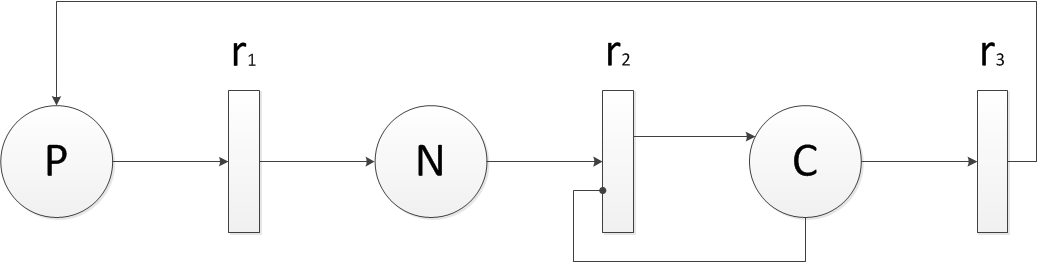
\includegraphics[width=10cm]{../resources/images/petri1.png}
	\label{petri1}
	\caption{Rete di petri per modellare l'accesso ad una risorsa condivisa}
\end{figure}

\subsection{Definizione degli stati del sistema}

Il modulo utente deve, ovviamente, importare il modulo CTMC, per la definizione
della sintassi del modello.
\begin{Verbatim}[fontsize=\small]
mod CTMC-PETRI_CONCURRENT is
   pr CTMC .
\end{Verbatim}

Uno state CTMC è definito come un contenitore di un operatore polimorfico,
dunque è possibile inserire un qualunque Sort definito od importato all'interno
del modulo utente.
\begin{Verbatim}[fontsize=\small]
op <_> : Universal -> State [ ctor poly (1) ] .
\end{Verbatim}
Supponendo di voler gestire lo stato del sistema come un multi-set di stringhe
che rappresentano i token della rete di Petri si può definire un Sort in questo
modo:
\begin{Verbatim}[fontsize=\small]
sort PetriState Token .
subsort String < Token < PetriState .
op nil : -> PetriState [ ctor ] .
op __ : PetriState PetriState -> PetriState [ ctor comm assoc id: nil ] .
\end{Verbatim}
Ottenendo una rappresentazione dello stato ad esempio con 2 token in $p$ ed 1 in
$n$:
\begin{Verbatim}[fontsize=\small]
< "p" "p" "n" >
\end{Verbatim}

\subsection{Definizione del modello}

Un modello CTMC descritto da un insieme di transizioni $State \Longrightarrow [Rate] State$ $if$
$Condition$, dove $State$ uno lo stato del sistema, $Rate$ è il rate con cui
scatta la transizione e $Condition$ è un requisito necessario perché la
condizione scatti.

Il framework richiede che il modello sia espresso come una serie di \emph{rule}
di \emph{rewrite} con etichetta \emph{model}, che riscrivono uno
\emph{State} in un \emph{Config}. Un $Config$ è una combianzione di $Rate$ +
$State$, così definito:
\begin{Verbatim}[fontsize=\small]
op [_]_ : Rate State -> Config [ ctor prec 80 ] .
\end{Verbatim}
Dunque le rule da scrivere assumono la forma:
\begin{Verbatim}[fontsize=\small]
rl [model] : State => [ Rate ] State.
\end{Verbatim}
oppure
\begin{Verbatim}[fontsize=\small]
crl [model] : State => [ Rate ] State if Condition .
\end{Verbatim}
Scegliendo dei rate per le varie transizioni (ad esempio $r1 \rightarrow 10$,
$r2 \rightarrow 24$ e $r3 \rightarrow 5.2$) si costruisce facilmente il modello:

\begin{Verbatim}[fontsize=\small]

op notC : PetriState -> Bool .
eq notC("c" P:PetriState) = false .
eq notC(P:PetriState) = true [ owise ] .
	
rl [model] : < "p" P:PetriState > => [ 10.0 ] < "n" P:PetriState > .
crl [model] : < "n" P:PetriState > => [ 24.0 ] < "c" P:PetriState >
        if  notC(P:PetriState) .
rl [model] : < "c" P:PetriState > => [ 14.2 ] < "p" P:PetriState > .

\end{Verbatim}
L'arco inibitore è stato modellato come una condizione all'interno della rule,
risolta dall'operazione \emph{notC}.

\emph{Nota:} grazie al mapping fra il modello CTMC e le rule di Maude, è
possibile sfruttare il matching nativo in qualunque punto della rule, ad esempio
creando rate dipendenti dallo stato del sistema.

\subsection{Gestione dell'Overview}

Durante la simulazione può essere utile voler ricevere delle informazioni
periodiche sulla dinamica del sistema per poter stampare a video delle
informazioni aggiuntive tramite l'attributo $print$ \cite{maudemanual}, che si
abilita con il comando Maude:
\begin{Verbatim}[fontsize=\small]
Maude> set print attribute on .
\end{Verbatim}

All'avvio della simulazione, è possibile specificare ogni quanti passi di
simulazione ricevere l'overview. Overview è un contenitore di una lista di
coppie $(tempo, stato)$ e rappresenta l'evoluzione del sistema nel tempo.
\begin{Verbatim}[fontsize=\small]
	sort Overview Entry EntryList .
	subsort Entry < EntryList .
	
	op _:_ : Float State -> Entry [ ctor prec 80 ] .
	op empty : -> EntryList [ ctor ] .
	op _ - _ : EntryList EntryList -> EntryList [ ctor assoc id: empty prec 90 ] .
	op [_] : EntryList -> Overview [ ctor ] .
\end{Verbatim}
Durante la simulazione, l'engine, ogni volta che compie il numero di passi
specificato, effettua una rewrite con profondità 1 dell'Overview sul modulo
utente. Quindi nel modulo utente deve essere presente una rule che trasformi in
un solo passo l'overview in un nuovo overview a cui si appenderanno le
\emph{Entry} successive. Nel contempo si può sfruttare questa rewrite stampando
a video le informazioni desiderate, ricordando che un termine è in ogni caso
completamente ridotto prima di essere descritto (in pratica sono eseguiti tutti
i sistemi di equazioni).

Ad esempio per questa rete potrebbe essere interessante elaborare le
informazioni per contare il numero di accessi alla risorsa condivisa:
\begin{Verbatim}[fontsize=\small]
	var EL : EntryList .
	var T1 T2 : Float .
	var S : State .
	var N N1 N2 : Nat .
	var P1 P2 P3 : PetriState .
	
	op print : EntryList -> EntryList .
	op countAccess : EntryList -> Nat .
	
	*** Riscrivo l'overview come il risultato dell'operazione print
	rl [overview] : [EL] => [ print(EL) ] .
	
	eq print(empty) = empty .
	ceq print(EL - T1 : S) = T1 : S
	  if   N := countAccess(EL - T1 : S) [ print "Numero accessi = " N ] .
	
	
	eq countAccess(empty) = 0 .
	ceq countAccess(T1 : < P1 > - T2 : < "c" P2 >  - EL) =
	                1 + countAccess(EL) if notC(P1) .
	eq countAccess(T1 : < P1 > - EL) = countAccess(EL) [ owise ] .
\end{Verbatim}

\section{Avviare una simulazione}

Una simulazione consiste nella riduzione dell'operazione \emph{simulate}
all'interno del modulo \emph{CTMC-ENGINE}, passando come argomenti:
\begin{description}	
\item[Qid:] Nome del modulo utente.
\item[Term:] meta-stato iniziale: la meta rappresentazione è ottenibile con
l'operazione \emph{upTerm}.
\item[Nat:] Numero di passi di simulazione desiderati.
\item[Nat:] Ogni quanti passi ricevere l'overview (0 se non si vuole ricevere
l'Overview).
\item[Nat:] Indice per la generazione dei numeri random da cui iniziare.
\end{description}

L'ultimo argomento è essenziale a causa della gestione della generazione dei
numeri casuali di Maude. Maude utilizza un algoritmo che genera sequenze di
numeri casuali partendo da un seed. Il seed lo si specifica all'avvio di maude,
eseguendo il comando:
\begin{Verbatim}[fontsize=\small]
$ maude -random-seed=number
\end{Verbatim}
dove $number \in [0, 2^{32} - 1]$ (di default vale 0); mentre l'indice della
sequenza è specificato all'esecuzione dell'operazione \emph{rand}. Per non dover
riavviare Maude ad ogni simulazione, basta cambiare l'ultimo argomento della
\emph{simulate}.

Ad esempio per eseguire una simulazione sul modulo creato in precedenza
($CTMC-PETRI\_CONCURRENT$), con stato iniziale di 4 token nel place $p$,
eseguendo 10000 passi di step e ricevendo l'overview ogni 1000 si può realizzare con il
comando:
\begin{Verbatim}[fontsize=\small]
Maude> reduce in CTMC-ENGINE : simulate('CTMC-PETRI_CONCURRENT ,
   '<_>['__['"p".Char '"p".Char '"p".Char '"p".Char ]] , 10000, 1000, 0) . 
\end{Verbatim}
La specifica dello stato iniziale può essere difficoltosa, quindi si consiglia
di creare un modulo di wrapping che import sia CTMC-ENGINE che
CTMC-PETRI\_CONCURRENT e che costruisca il meta-stato:
\begin{Verbatim}[fontsize=\small]
mod CTMC-PC_SIMULATOR is
  pr CTMC-PETRI_CONCURRENT .
  pr CTMC-ENGINE .
  
  op simulate : Nat Nat Nat -> SimulationResult .
  eq simulate(S:Nat, O:Nat, R:Nat) =
     simulate('CTMC-PETRI_CONCURRENT , upTerm( < "p" "p" "p" "p" > ), S:Nat,
              O:Nat, R:Nat ) .  
endm
\end{Verbatim}

La simulazione termina o al compimento di tutti i passi richiesti, o al
raggiungimento di un deadlock (in questo caso non sono presenti deadlock). Il
valore di ritorno di una simulazione è un \emph{SimulationResult}:
\begin{Verbatim}[fontsize=\small]
*** SimulationResult -> composto da tempo + risultato finale + deadlock?
sort SimulationResult .
op sim : Float State Bool -> SimulationResult [ ctor ] .
\end{Verbatim}

\section{Verifica di proprietà}

Una vola definito il modello, è possibile utilizzare l'APMC per verificare
proprietà espresse da formule PCTL monotone, ovvero formule contenenti operatori
\emph{next} e \emph{until} bounded e non, \emph{implies}, \emph{false} e
verifica che la probabilità di queste formule sia maggiore o uguale ad un dato
valore. La grammatica (a scopo $\phi$) per tali formule è:
 \[
\phi ::= p | FALSE | \phi \rightarrow \phi' | P_{\geq J}[\psi]
\]
\[
\psi ::= X \phi | \phi U \phi' | \phi U^I \phi'
\]

\subsection{Scrittura di formule PCTL}

Queste formule sono rappresentate nel modulo \emph{PCTL}. Il sort \emph{Formula}
identifica le $\phi$, mentre il sort \emph{PathFormula} identifica le $\psi$.
\begin{Verbatim}[fontsize=\small]
*** Formula -> phi ; PathFormula -> psi
sort Formula PathFormula .

*** Un predicato p è un meta-stato.
subsort Term < Formula .
*** p(Term, Condition) effettua un matching di Term con lo stato corrente,
*** controllando la Condition.
op p : Term Condition -> Formula [ ctor ] .
op FALSE : -> Formula [ ctor ] .
op TRUE : -> Formula [ ctor ] .
op _ implies _ : Formula Formula -> Formula [ ctor prec 90 ] .
op _ and _ : Formula Formula -> Formula [ ctor prec 80 ] .
op _ or _ : Formula Formula -> Formula [ ctor prec 80 ] .
op not _ : Formula -> Formula [ ctor prec 75 ] .
op P[_](_) : Float PathFormula -> Formula [ ctor prec 70] .

op (_)U[_](_) : Formula Float Formula -> PathFormula [ ctor prec 92] .
op (_)U(_) : Formula Formula -> PathFormula [ ctor prec 92] .
op X_ : Formula -> PathFormula [ ctor ] .
\end{Verbatim}

Il predicato $p$ della grammatica è uno meta-stato Term, e semanticamente
significa: $p \equiv S$, dove $S$ è il meta-stato corrente. Per aggiungere più
espressività ai predicati, si può utilizzare l'operatore \emph{p(State, Condition)}, dove il
secondo argomento è una condizione espressa sul meta-stato con sintassi
definita dal sort \emph{Condition}.

Ad esempio si può esprimere la formula che si avveri se non c'è nessun token nel
place $p$. Una operazione per verificarla potrebbe essere la seguente:
\begin{Verbatim}[fontsize=\small]
op notP : PetriState -> Bool .
eq notP("p" P:PetriState) = false .
eq notP(P:PetriState) = true [ owise ] . 
\end{Verbatim}
Quindi vorremmo scrivere qualcosa del tipo
\begin{Verbatim}[fontsize=\small]
if notP(P:PetriState) = true
\end{Verbatim}
Questa condizione deve essere espressa come sort \emph{Condition}, diventando:
\begin{Verbatim}[fontsize=\small]
'notP['P:PetriState ] = 'true.Bool
\end{Verbatim}

Con un esempio più completo: è vero che non c'è più nessun processo nello stadio
di partenza in almeno 1.75 unità di tempo con una probabilità maggiore del
$40\%$? \begin{Verbatim}[fontsize=\small]
P[0.4]( ( TRUE ) U[1.75] (
   p( '<_>[ 'P:PetriState ] , 'notP['P:PetriState ] = 'true.Bool )))
\end{Verbatim}

\subsection{Verifica di formule PCTL}

La verifica di formule PCTL avviene sempre nel modulo \emph{PCTL}, con la
tecnica APMC, che permette di ottenere soluzioni che appartengono al range
($[\nu - \epsilon ; \nu + \epsilon$) entro una certa confidenza
$(1 - \delta)$, dove $\nu$ è la probabilità esatta. La verifica si compie
riducendo l'operazione \emph{verify}, che accetta i seguenti argomenti:
\begin{description}
\item[Qid:] Nome del modulo utente su cui c'è il modello .
\item[Formula:] formula PCTL fa verificare
\item[Term:] meta-stato iniziale
\item[Float:] Approximation ($\epsilon$)
\item[Float:] Confidence ($\delta$)
\item[Nat:] Max Depth (profondità massima delle path da generare).
\item[Nat:] indice di partenza per la generazione di numeri casuali
\end{description}

Ad esempio la verifica della formula precedente con $\epsilon = 0.2$
e $\delta = 1.0\cdot10^{-2}$, con una profondità massima di 10000:

\begin{Verbatim}[fontsize=\small]
reduce in PCTL : verify('CTMC-PETRI_CONCURRENT , 
          P[0.4]( ( TRUE ) U[0.49999] (
          p( '<_>[ 'P:PetriState ] , 'notN['P:PetriState ] = 'true.Bool ))) ,
          '<_>['__['"p".Char '"p".Char '"p".Char '"p".Char ]] ,
       0.2, 0.01, 10000 , 0) .
\end{Verbatim}

Come per la simulazione, anche in questo caso conviene realizzare un modulo di
wrapping per evitare di scrivere a mano gli State al meta-livello:
\begin{Verbatim}[fontsize=\small]
mod CTMC-PC_VERIFIER is
  pr CTMC-PETRI_CONCURRENT .
  pr PCTL .
  
  op verify : Formula Float Float Nat Nat -> Bool .
  eq verify(F:Formula, app:Float, conf:Float, dep:Nat, R:Nat) =
     verify('CTMC-PETRI_CONCURRENT , F:Formula , upTerm( < "p" "p" "p" "p" > ),    		  
        app:Float, conf:Float, dep:Nat, R:Nat ) .  
endm
\end{Verbatim}
e poi nella console di Maude:
\begin{Verbatim}[fontsize=\small]
reduce in CTMC-PC_VERIFIER : verify(
          P[0.4]( ( TRUE ) U[0.49999] (
          p( upTerm( < P:PetriState > ) , 'notP['P:PetriState] =
          'true.Bool ))) , 0.2, 0.01, 10000 , 0) .
\end{Verbatim}
Attenzione ad usare bene l'upTerm, tenendo conto che prima di salire al
meta-livello, un termine è completamente ridotto ove possibile.
